% !TeX encoding = UTF-8
% !TeX spellcheck = en_US
% !TeX root = presentation.tex

\section{Introduction}
\begin{frame}{Software Development Project}
\end{frame}

\begin{frame}{Basic Navigation Test}
\begin{itemize}
    \item Environment: Workspaces, waypoints and obstacles.
    \item Task specification: Sequence of poses.
\end{itemize}
\centering 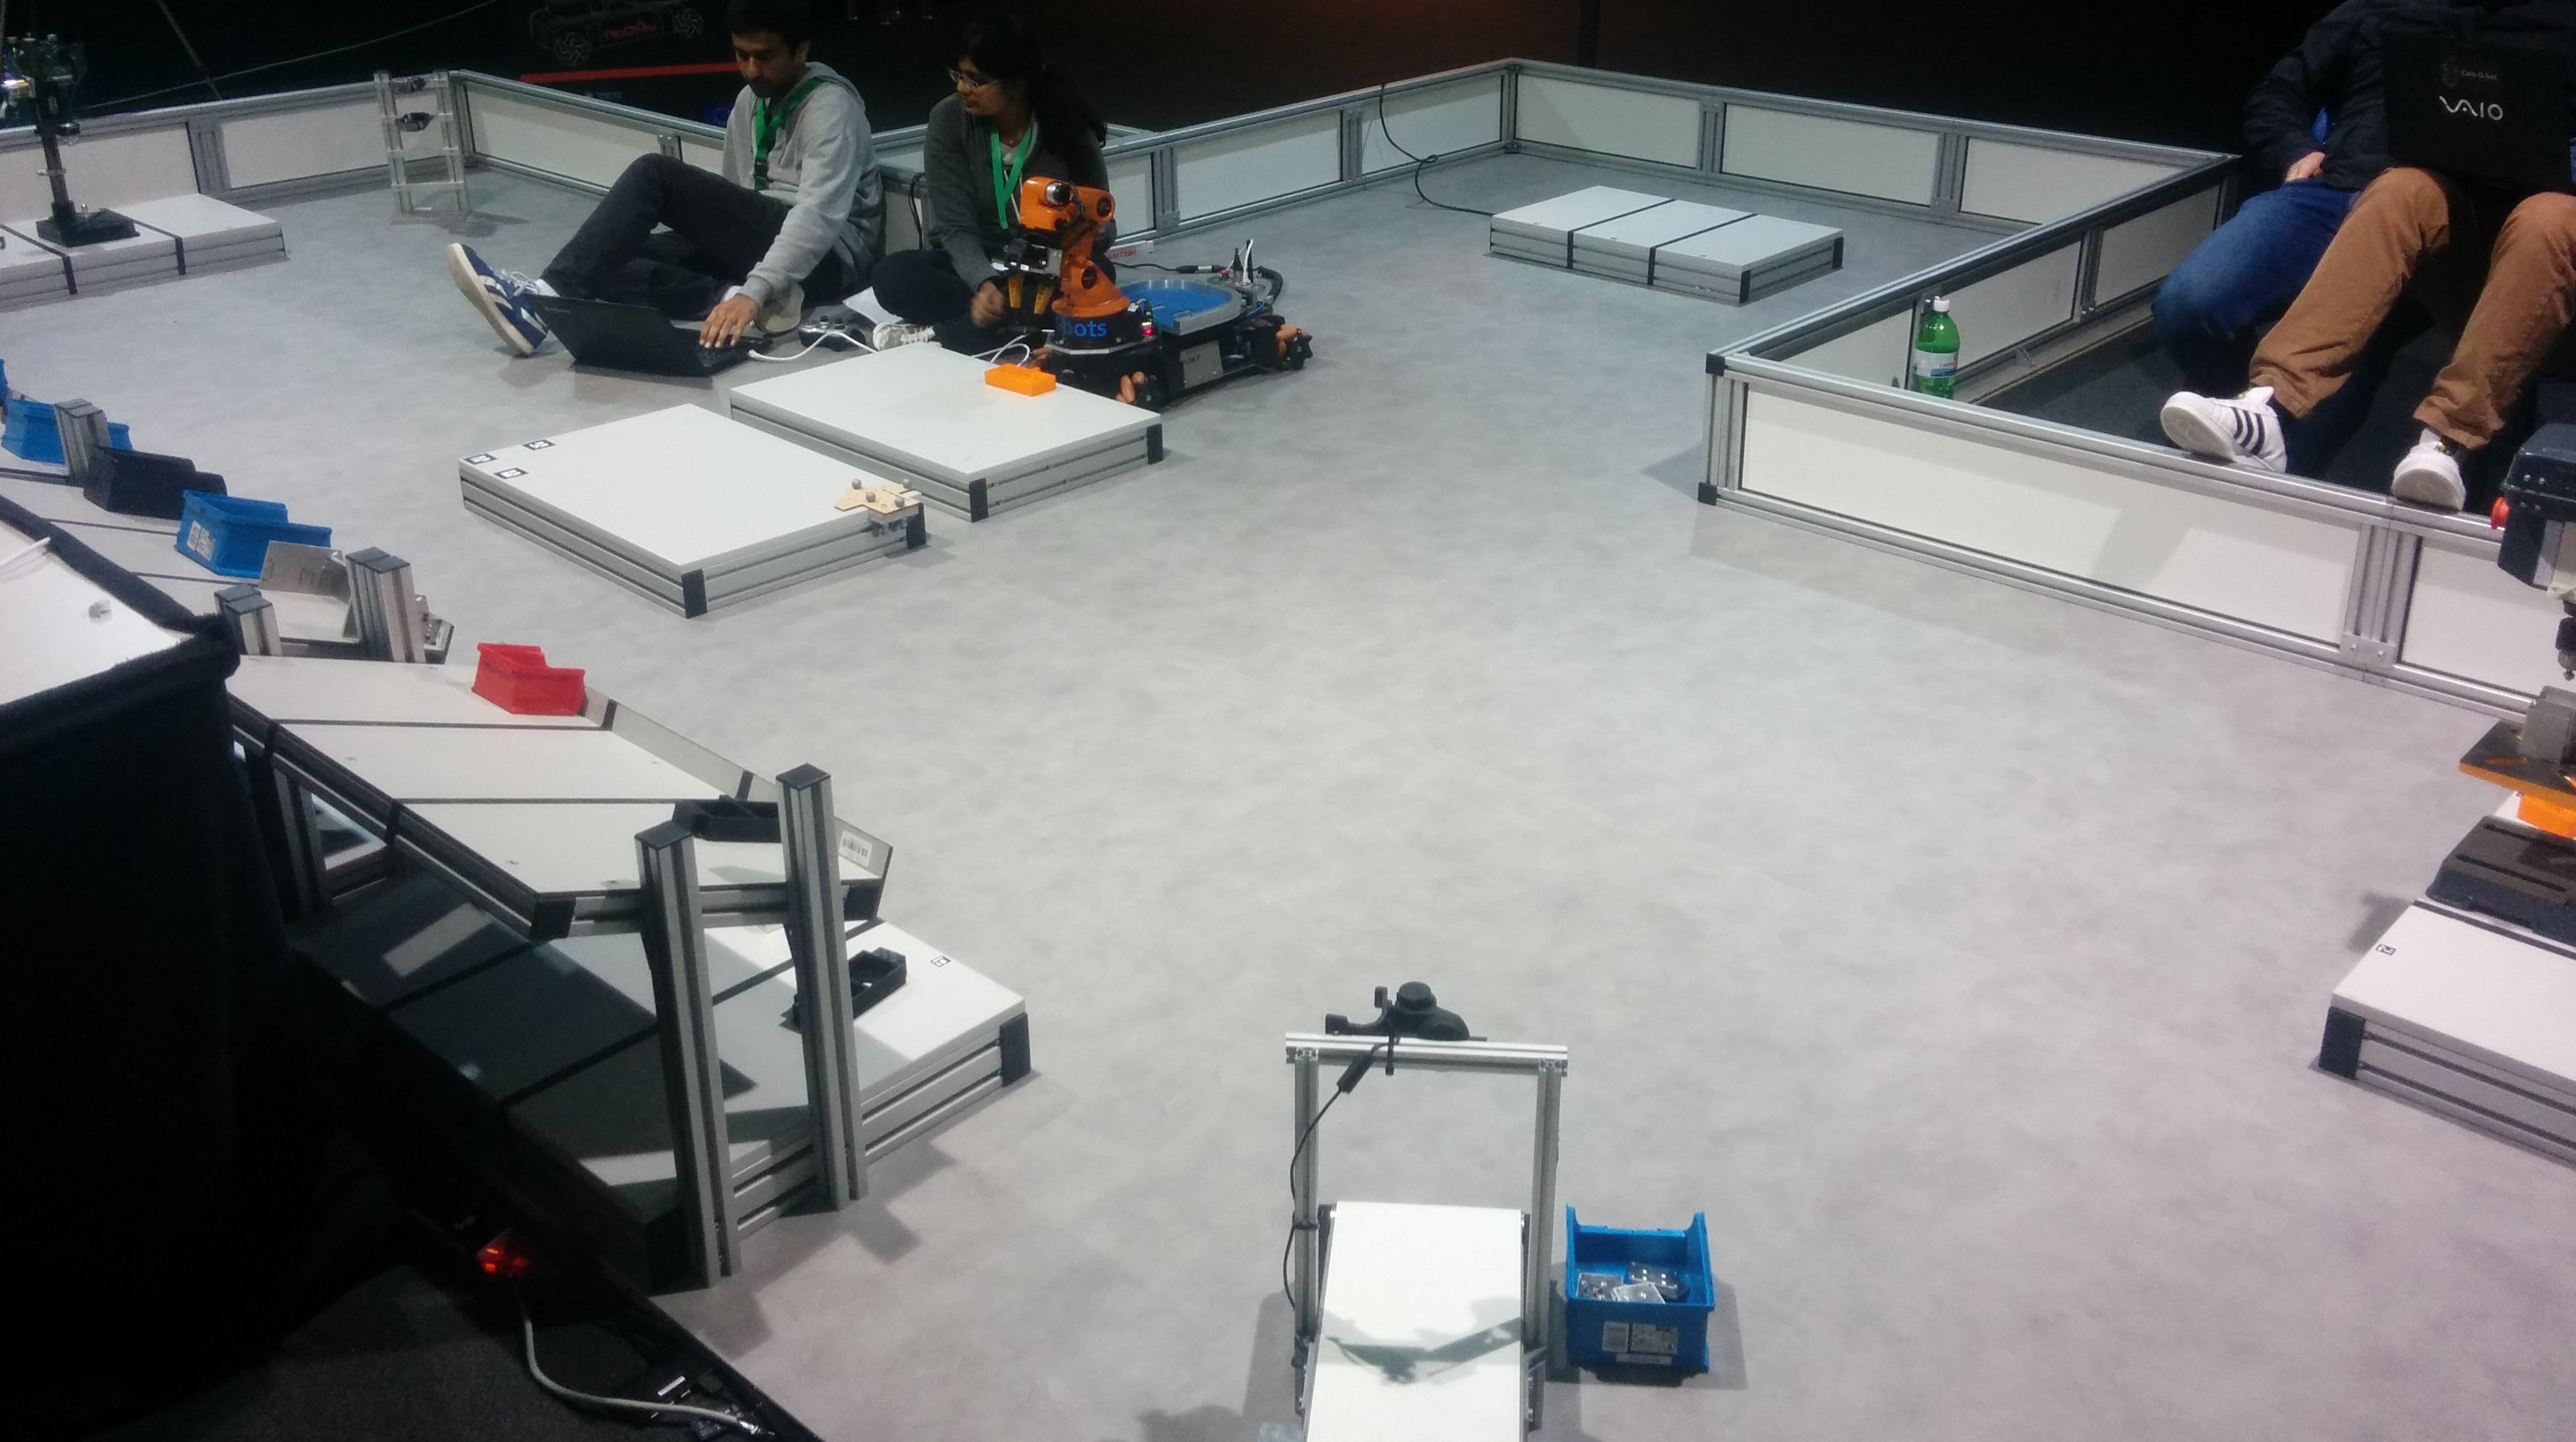
\includegraphics[height=50mm]{gfx/arena.jpg}
\end{frame}

\begin{frame}{Challenges}
\begin{itemize}
    \item \textbf{Perception:} Accessing and processing sensor data.
    \item \textbf{Mapping:} Building map of the environment.
    \item \textbf{Localization:} Pose inside map.
    \item \textbf{Path planning:} Determine sequence of poses between waypoints.
    \item \textbf{Motion control:} Execution of path.
\end{itemize}
\end{frame}

\begin{frame}{KUKA youBot}
The youBot is a mobile manipulator designed for education and research purposes. It comes with fully open interfaces and API. 
\begin{columns}
    \begin{column}{0.6\textwidth}
        %\begin{block}{System}
        \begin{itemize}
            \item Omnidirectional, four-wheeled
            \item 5-DOF manipulator with a two-finger gripper
            \item On-board PC with CPU, 2GB memory, 32GB SSD drive
            \item Sensors: vision sensors, rangefinders
        \end{itemize} 
        %\centering \includegraphics[width=0.25\textwidth]{slides/gfx/youbot.jpg}   
        %\end{block}
    \end{column}
    \begin{column}{0.4\textwidth} % alternative top-align that's better for graphics
        \centering
        \includegraphics[width=\linewidth]{gfx/youbot.jpg}
    \end{column}
    
\end{columns}
\end{frame}

\begin{frame}{Robot Operating System (ROS)}
Set of software and libraries.
\begin{itemize}
    \item \textbf{Node}: A process using ROS. 
    \item \textbf{Topic}: Message queue, used for communication between nodes.
    \begin{figure}
        
\includegraphics[width=0.5\textwidth]{gfx/topic.png}
    \end{figure}
    \item \textbf{Service}: Offers synchronous service calls.
    \begin{figure}
        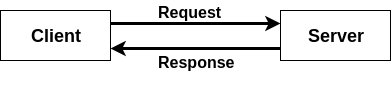
\includegraphics[width=0.5\textwidth]{gfx/service.png}
    \end{figure}
\end{itemize}
\end{frame}